%!TEX root = ./main.tex
%!TEX encoding = UTF-8 Unicode

\chapter{Interrupt description}
\label{chap:interrupt}
\section{Introduction}
This chapter describes how interrupts are handled in the Harmless language, and more precisely how an interrupt handler is described. This is done in 2 steps:
\begin{itemize}
\item first, an interrupt is generated either by a peripheral (see chapter \ref{chap:peripherals}), or by software.
\item Then hardware interrupt controller get the interrupt and perform the associated behavior (pushing the program counter for instance). The way the interrupt vector is handled is described in this interrupt controller.
\end{itemize}

\section{Hardware Interrupt Description}
The hardware interrupt controller is a simple method of a component. This method should have the following prototype:
\begin{lstlisting}
void hardInterruptHandler(u32 trapId)
\end{lstlisting}
It does not return any value, and the parameter is given by the interrupt source (\emph{trap} or \emph{source} number). The name of the method does not care. In order to make Harmless use this method as the target for interrupt requests, it \emph{should} be declared in the \texttt{default} section, like this:
\begin{lstlisting}
default {
    -- ...
    interrupt := it.hardInterruptHandler
}
\end{lstlisting}
In this example, interrupts requests will be routed to the method \texttt{hardInterruptHandler} of component \texttt{it}.

An interrupt request may be done either in a component (peripheral for instance) or a behavior (software interrupt) (see section \ref{keyword:interrupt})
\begin{lstlisting}
    interrupt 5
\end{lstlisting}
In this example, \texttt{5} is the \texttt{trapId} parameter that may be used in the hardware interrupt controller.
\section{A full Example}
Here is an example based on the Atmel AVR. First, we declare an hardware interrupt controller in the default section of Harmless:
\begin{lstlisting}
default {
    -- ...
    interrupt := it.hardInterruptHandler
}
\end{lstlisting}

Our interrupt description restricts to the default one: The interrupt vector starts at address 0, and requires 2 bytes for each entry (figure \ref{fig:itAVR}).
\begin{figure}[h]	
  \begin{center}
    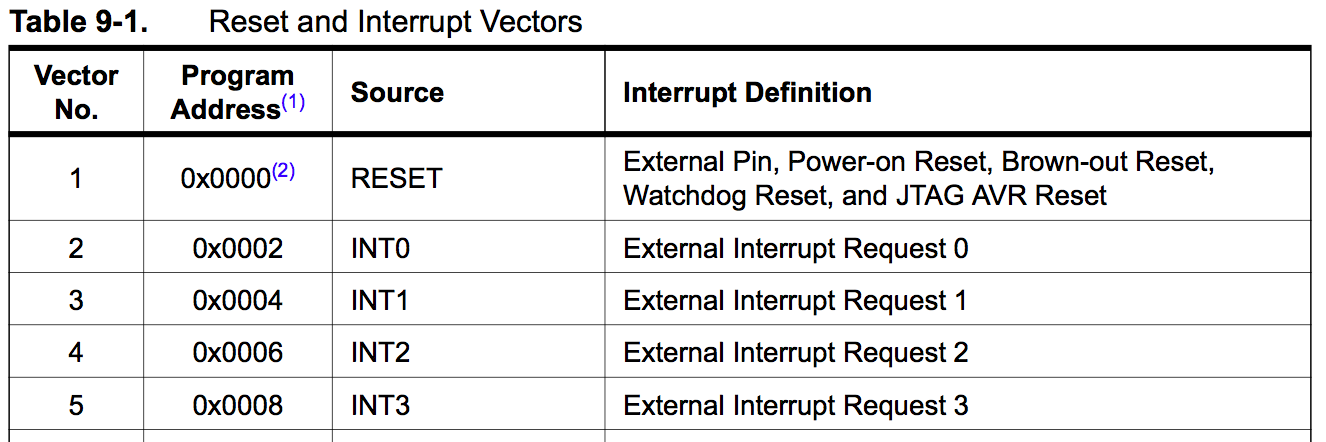
\includegraphics[width=0.95 \linewidth]{../common/images/exampleInterruptVectorAVR.png}
    \caption{First entries in the interrupt Vector for the Atmel AVR® \emph{Source Atmel}}
    \label{fig:itAVR}
  \end{center}
\end{figure}
In our description, we use the \texttt{program address} as the \texttt{trapId} to differentiate interrupt sources.

The description of the interrupt controller is:
\begin{lstlisting}
  void hardInterruptHandler(u32 trapId) {
    if CCR.I then -- global mask    
      -- push current PC: no information about the way PC is stored (same as CALL)
      sram.push(PC{8..1})  --as PC is on 17 bits
      sram.push(PC{16..9})
      -- then branch.
      Fetcher.absBranch((s16)(trapId))
    end if
  }
\end{lstlisting}
It first checks that the global interrupt mask is set (the local mask should be tested before). Then it pushes the program counter (PC) and branches to the appropriate interrupt vector entry. This entry should be a jump instruction to the software interrupt handler. 

There is an example of \emph{timer} using interrupts in chapter \ref{chap:peripherals}.


WARNING: This approach does NOT differ interrupts! In this description, if CCR.I is not set, the interrupt WON'T occur.